\section{Electrical}

\subsection{Power Distribution}
The ASV is powered by two 12.8V 8Ah LiFePO4 batteries connected in parallel. A \SI{100}{\watt} solar panel mounted above the electronics enclosure outputs power to an MPPT controller, which continuously regulates the voltage and current to maximize the power output from the solar panel. The charge controller adjusts the variable DC that comes in from the solar panel to a constant voltage and current that is suitable for charging the batteries. The MPPT controller outputs the current through Anderson Powerpole connectors, which are tied into the circuit via a 12p junction terminal block, which distributes power to the rest of the system. The use of Anderson connectors allows for easy connection and disconnection of the solar panel. The batteries are connected with F2 spade connectors, also allowing for easy connection and disconnection.

Power is distributed through two voltage regulators that step the 12.8V battery voltage down to 5V. One converter supplies the SpeedyBee F405 V4 flight controller and GPS, and the other is dedicated to the servo motor. All components are placed inside a waterproof enclosure without mounting hardware. Initially, the voltage regulator was a buck converter on a PCB, but was replaced with a voltage regulator on a perfboard. The buck converter was not able to handle the current draw of the Speedybee, which caused it to overheat and fail. 

% Miles should write the section about the buck converters and the PCB design, but include a schematic of the protoboard

\subsection{Flight Controller and GPS}
\begin{figure}[H]
    \centering
    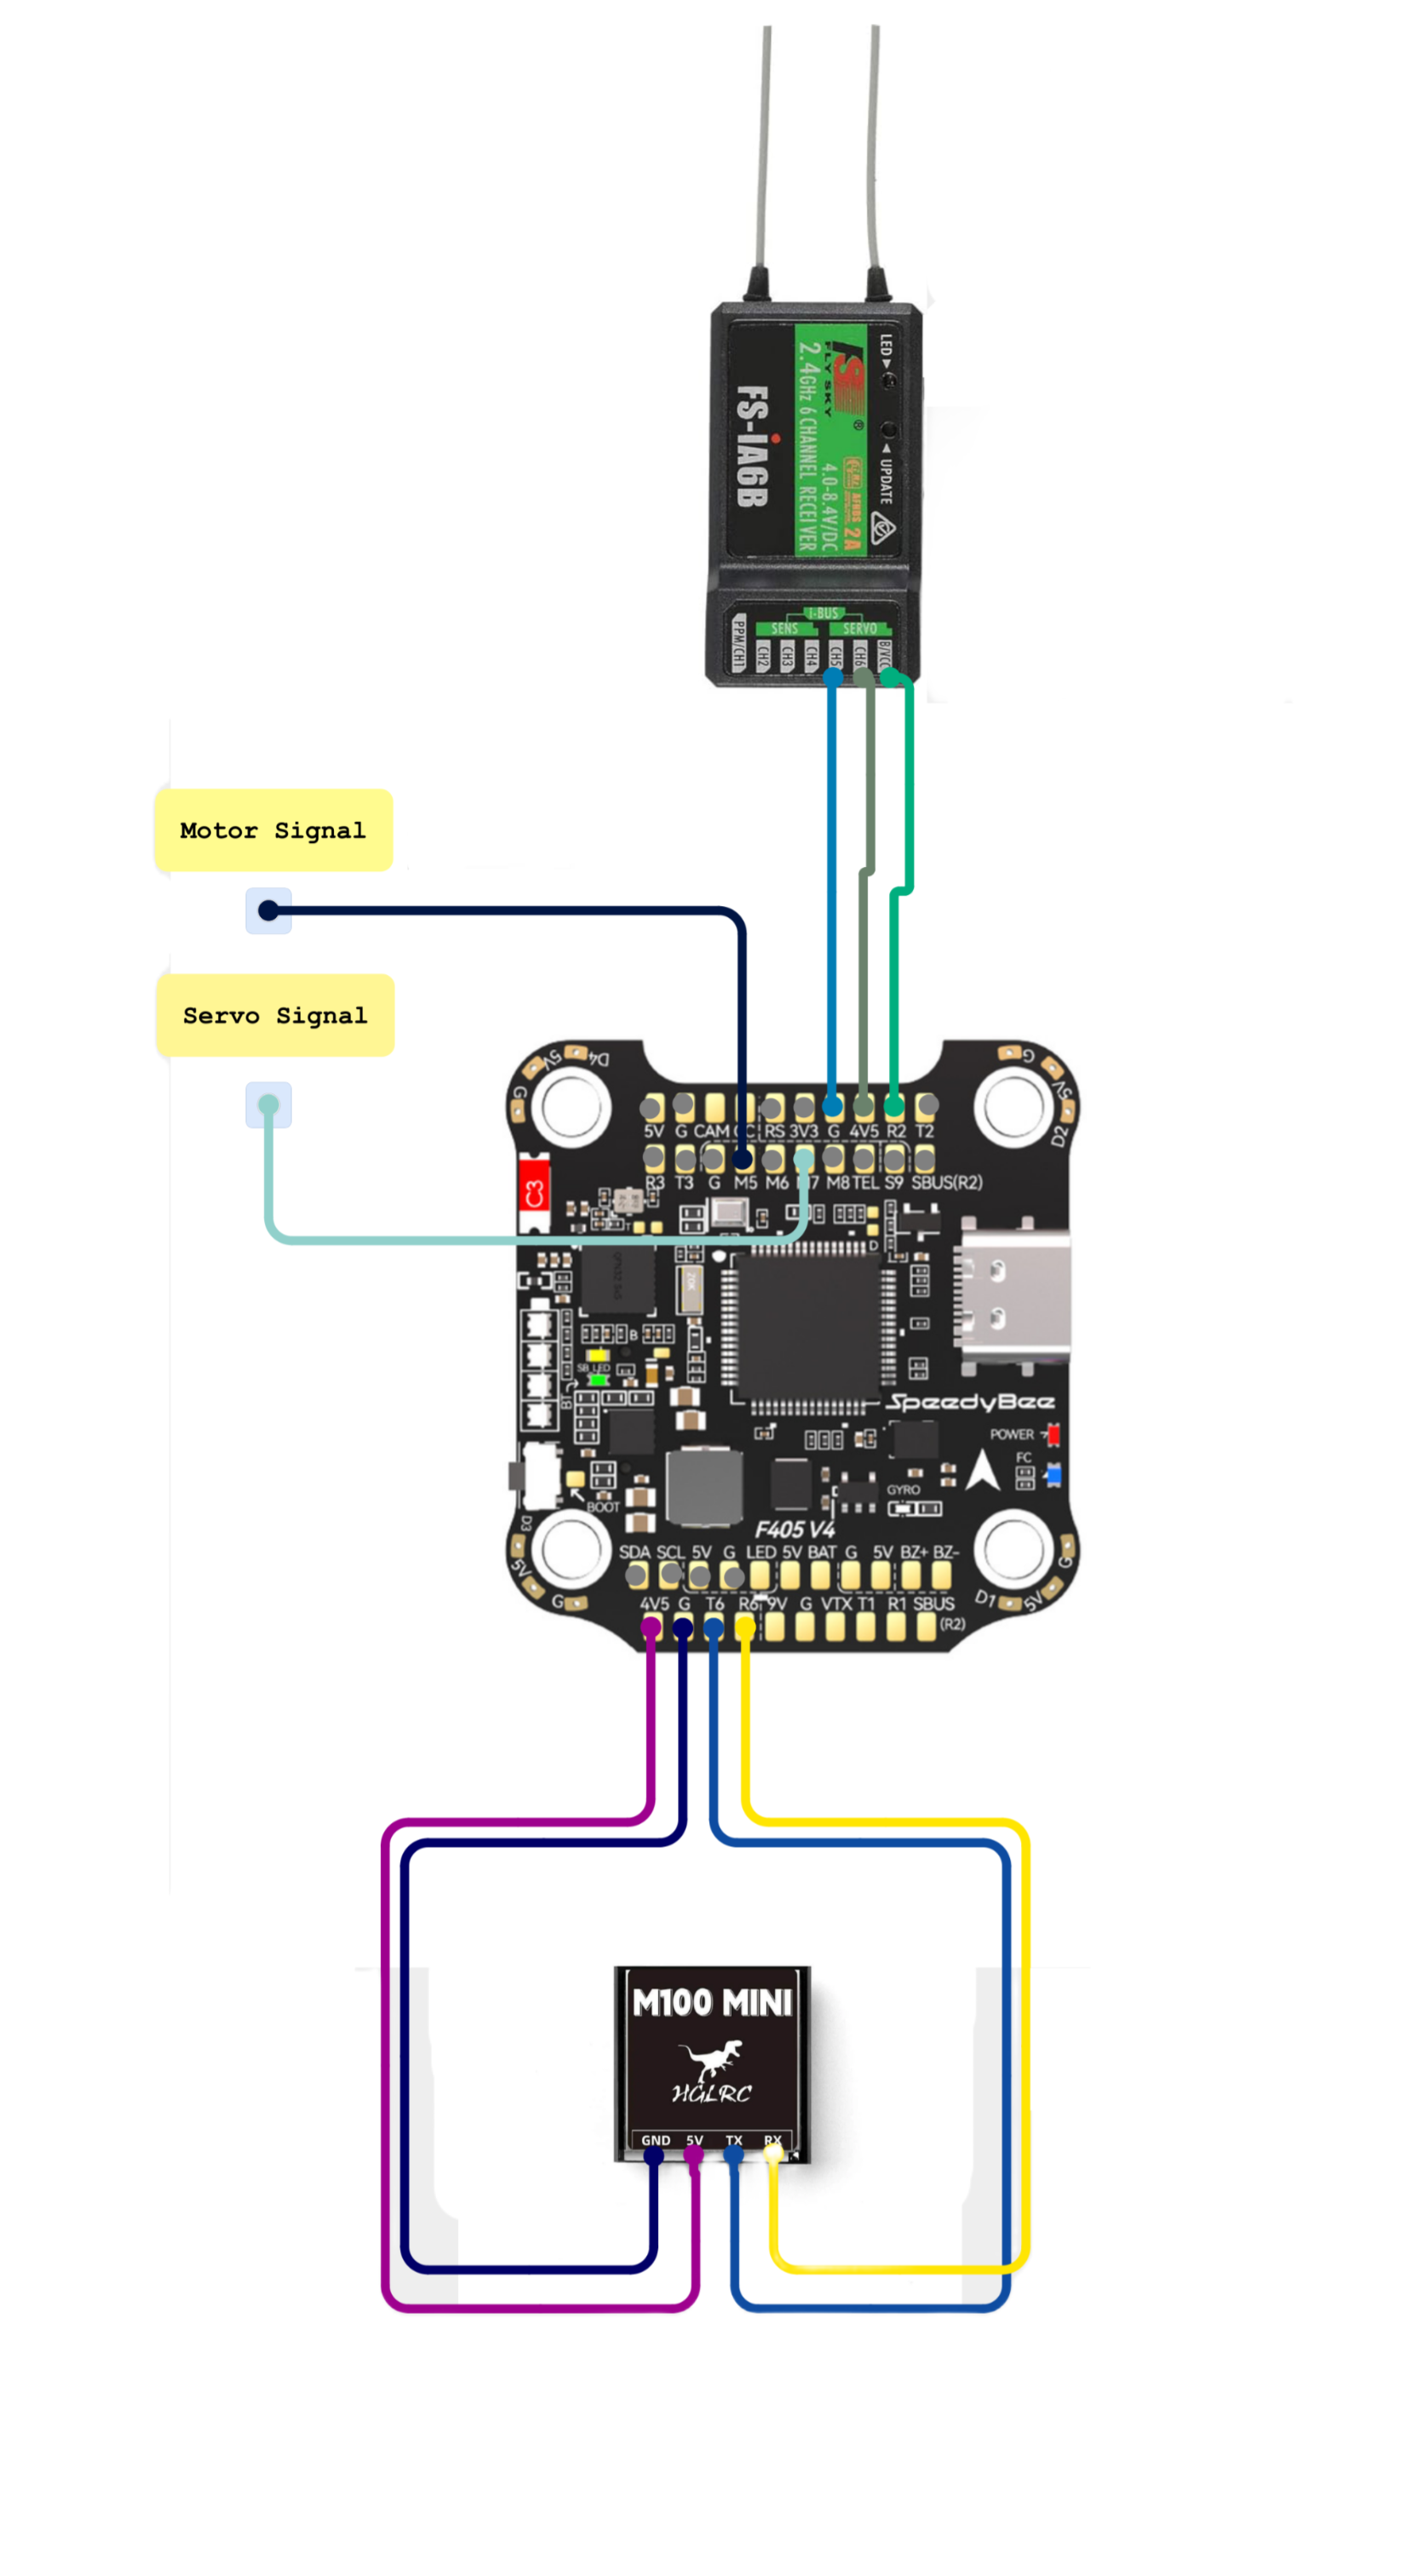
\includegraphics[height=10cm]{speedybee.png}
    \caption{Schematic of the SpeedyBee F405 V4 flight controller and its connections.}
    \label{fig:Speedybee}
\end{figure}

The SpeedyBee F405 V4 flight controller runs iNav firmware and handles both GPS waypoint navigation and motor control. It outputs PWM signals to the brushed DC motor and rudder servo and receives location data from a GPS module. The GPS is soldered directly to UART6 on the flight controller: TX from the GPS is connected to RX6, and RX from the GPS is connected to TX6. A FlySky FS-iA6B receiver is soldered directly to the RX2 pad on the flight controller for SBUS communication, enabling manual RC override when needed.

To generate a magnetic field, a 40 Hz sine wave is created by a prebuilt signal generator and passed through a power amplifier. The amplified signal drives a large copper coil wrapped around the boat’s structure, producing a low-frequency magnetic field detectable by submerged sensors.

The magnetic field \( B \) at the center of a circular coil is given by:

\begin{equation}
B = \frac{\mu_0 N I}{2R}
\label{eq:bfield}
\end{equation}

where:
\begin{itemize}
    \item \( \mu_0 = 4\pi \times 10^{-7} \, \text{T}\cdot\text{m/A} \) is the permeability of free space,
    \item \( N \) is the number of turns in the coil,
    \item \( I \) is the current through the coil,
    \item \( R \) is the radius of the coil.
\end{itemize}

This equation demonstrates that the magnetic field strength increases with more turns or higher current and decreases with a larger coil radius. The 40 Hz frequency was chosen to ensure good penetration through water with minimal signal loss, making it suitable for detection by submerged sensors.

All electrical connections are made using soldered wires. Power and signal lines are routed manually inside the enclosure. Signal and high-current paths are physically separated to minimize noise. Fuses are installed on the battery output lines to protect critical components from short circuits.

The electrical system is simple, modular, and designed for ease of repair and future upgrades. Components can be swapped or rewired without requiring full system disassembly.